\section{Technologie}
	\subsection{Client}
		\subsubsection{Sprache}
			\begin{tabularx}{\textwidth}{|lXX|}
				\hline
					\textbf{} & \textbf{Vorteile} & \textbf{Nachteile}\\
				\hline
					\textbf{JavaScript} & 
					\begin{itemize}
						\item UI der bestehenden Applikation ist auch in JavaSscript geschrieben
					\end{itemize} & 
					\begin{itemize}
						\item Fehler tauchen erst zur Runtime auf
					\end{itemize} \\
				\hline
					\textbf{TypeScript} &
					\begin{itemize}
						\item Wird kompiliert (zu Javascript), weniger Fehler zur Runtime
						\item Optisch besser lesbar als JavaScript
					\end{itemize} &
					\begin{itemize}
						\item Erfordert TSC-Compiler
						\item Code Overhead bei Inheritance
					\end{itemize} \\
				\hline
			\end{tabularx}
			
			
		\subsubsection{Architektur-Framework}
			\begin{tabularx}{\textwidth}{|lXX|}
				\hline
					\textbf{} & \textbf{Vorteile} & \textbf{Nachteile}\\
				\hline
					\textbf{Angular JS} &
					\begin{itemize}
						\item bekanntes MVW- und Templating Framework, erlaubt eine saubere Trennung von Logik und Darstellung
						\item bindet ViewModel Properties und Functions ans Template, wodurch sich Observerkonstrukte sparen lassen
						\item ist stabil, zuverlässig, gut erweiterbar und bringt von sich aus schon sehr viel mit
						\item wurde auch schon für die bestehende Applikation eingesetzt
					\end{itemize} &
					\begin{itemize}
						\item Attribute Binding besitzt gewissen Overhead
					\end{itemize} \\
				\hline
					\textbf{Ember JS} &				
					\begin{itemize}
						\item Sehr Modular und anpassbar
					\end{itemize} &
					\begin{itemize}
						\item Bringt wesentlich weniger mit als Angular JS, mehr Eigenaufwand notwendig
					\end{itemize} \\
				\hline
					\textbf{Kein Framework} &
					\begin{itemize}
						\item Vollständig freie Architekturgestaltung
					\end{itemize} &
					\begin{itemize}
						\item Hoher Implementationsaufwand ohne Gewinn
					\end{itemize} \\
				\hline
			\end{tabularx}
			
			\subsubsection{Require.js}
				Require.js eignet sich gut zur Strukturierung und zum Autolading der Klassen und komponenten, 
				insbesondere während der Entwicklung.

		\subsection{UI Frameworks}
			\subsubsection{LESS}
				Less soll als CSS Generator eingesetzt werden, da es den CSS Code stark verschlankt und Vorteile wie Variablen und Mixins bietet. LESS kann bei einem Node.js Server serverseitig compiled werden um den Client zu entlasten.
				
		\subsection{Testing}
			Testing Framework Anforderungen:
			\begin{itemize}
				\item Einfach einzubinden
				\item Einfach zu erweitern
				\item Bekannte Benutzung mit Tests und Asserts
				\item Möglichkeit zur Anbindung eines Build Tools
			\end{itemize}

			\subsubsection{JsUnit / QUnit}
				JsUnit wie QUnit arbeiten mit einem realen Browser (keine Browsersimulation), 
				sind einfach handzuhaben und bieten typische Assert-Syntax.
				
				
	\subsection{Server}

		\subsubsection{Evaluation}\label{serverEvaluation}
			Da die Servertechnologie eine grössere Entscheidung ist, haben wir sie ausführlich evaluiert.
			Zuerst haben wir gemeinsam Kriterien und mögliche Servertechnologien aufgelistet.
			Danach haben wir je separat die Gewichtung der Kriterien festgelegt sowie die Matrix Kriterium/Servertechnologie mit unserer Schätzung gefüllt, wie stark jede Servertechnologie das entsprechende Kriterium erfüllt.
		
			\begin{figure}[H]
				\begin{minipage}[b]{\linewidth}
					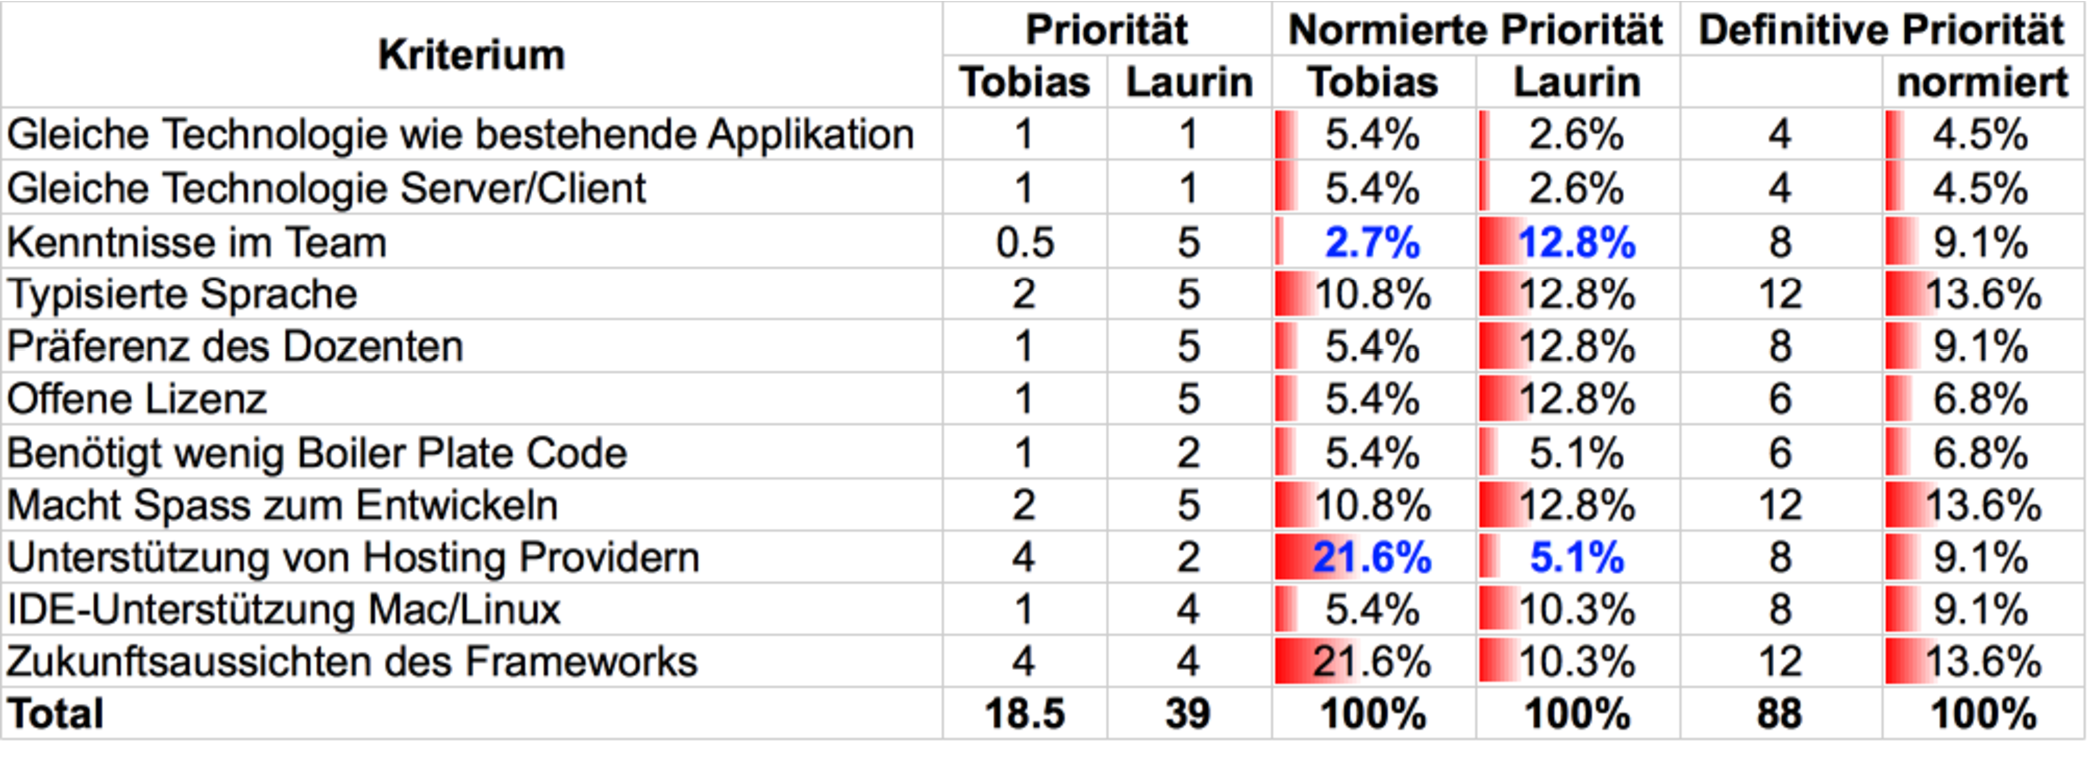
\includegraphics[width=\textwidth]{media/spreadsheets/ServertechnologieVergleichPrioritaetsfinding.pdf}
					\centering
					\caption{Servertechnologie-Vergleich: Prioritätsfinding}
					\label{fig:ServertechnologieVergleichPrioritaetsfinding}
				\end{minipage}
			\end{figure}
			
			In Abbildung~\ref{fig:ServertechnologieVergleichPrioritaetsfinding} sieht man den Prozess der Prioritätsfindung.
			Wie bereits erwähnt, haben wir zuerst die Kriterien definiert und anschliessend je separat Prioritäten für jedes Kriterium festgelegt.
			Da wir verschiedene Skalen verwendet haben, haben wir unsere Punkte noch zu 100\% normiert.
			Und aus diesen zwei Werten haben wir in gemeinsamer Diskussion die definitive Priorität erstellt.
			Dies hat meist problemlos funktioniert, ausser bei den Punkten "`Kenntnisse im Team"' und "`Unterstützung von Hosting Providern"' (blau markiert) hatten wir zu Beginn nennenswerte Differenzen.
			Bei diesen entsprechenden Punkten haben wir dann in der Diskussion gemerkt, dass wir uns wohl unter- oder überschätzt haben und wir haben uns dann auf ungefähr die Hälfte geeinigt.
		
			\begin{figure}[H]
				\begin{minipage}[b]{\linewidth}
					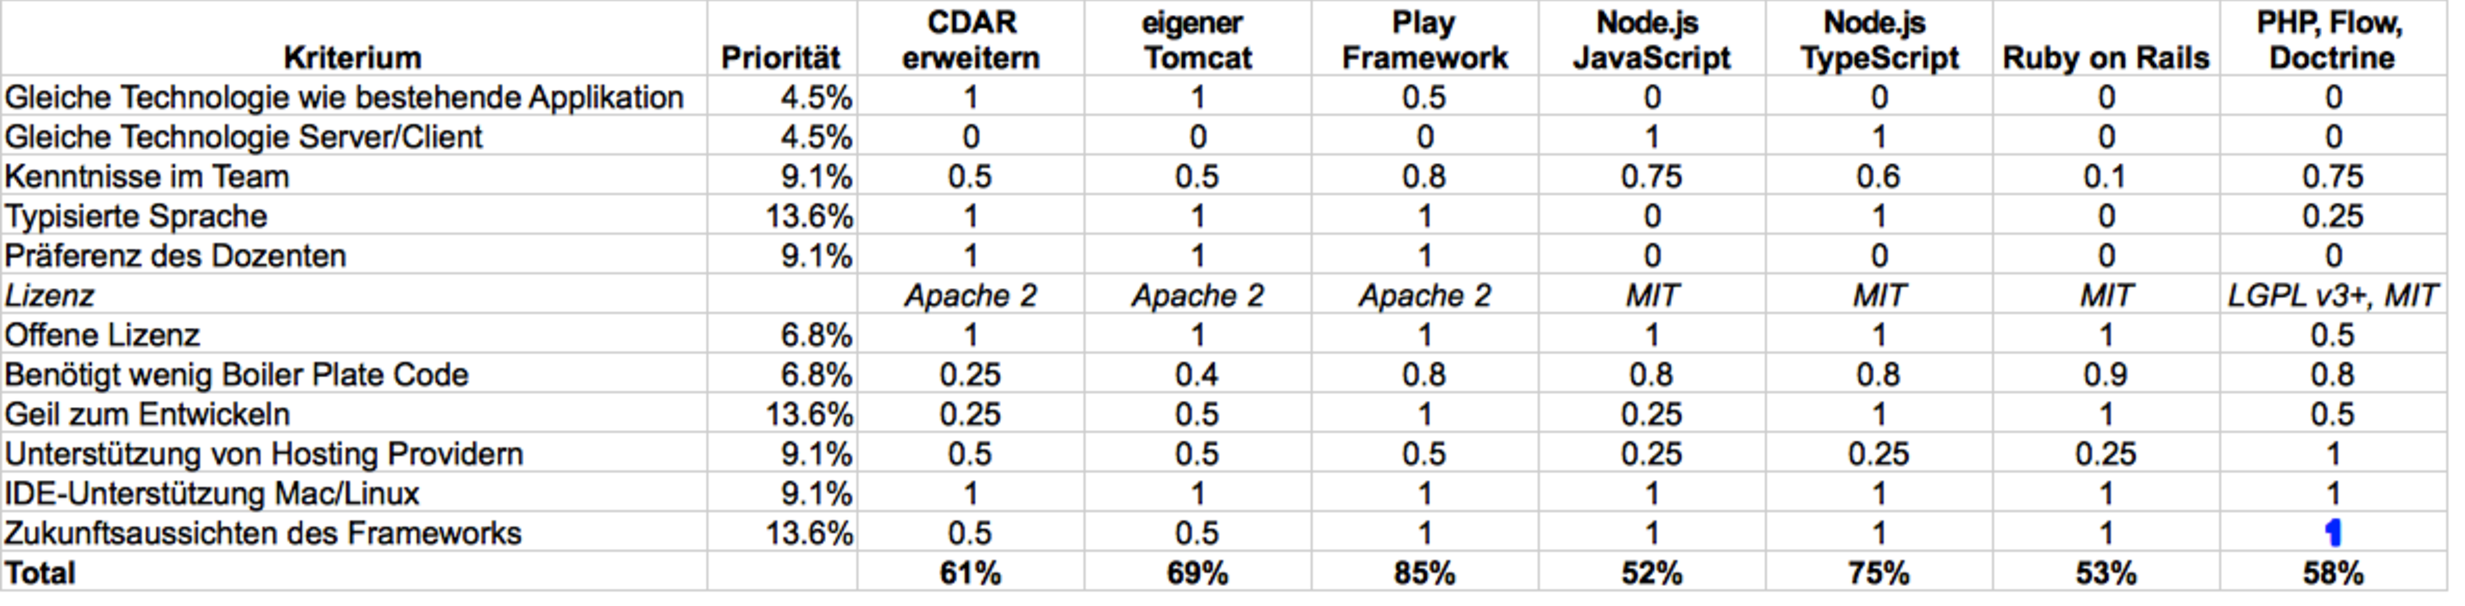
\includegraphics[width=\textwidth]{media/spreadsheets/ServertechnologieVergleichVergleichDerTechnologien.pdf}
					\centering
					\caption{Servertechnologie-Vergleich: Vergleich der Technologien}
					\label{fig:ServertechnologieVergleichVergleichDerTechnologien.pdf}
				\end{minipage}
			\end{figure}
			
			In Abbildung~\ref{fig:ServertechnologieVergleichVergleichDerTechnologien.pdf} sieht man den Vergleich der einzeln evaluierten Servertechnologien.
			Auch hier haben wir zuerst je separat die Schätzung gemacht und dann verglichen.
			Bei diesem Vergleich haben wir gar noch ähnlichere Werte gewählt, lediglich bei den Zukunftsaussichten von PHP, Flow und Doctrine (blau markiert) hatten wir eine nennenswerte Differenz.
			\begin{wrapfigure}{r}{0.618\linewidth}
				\begin{center}
					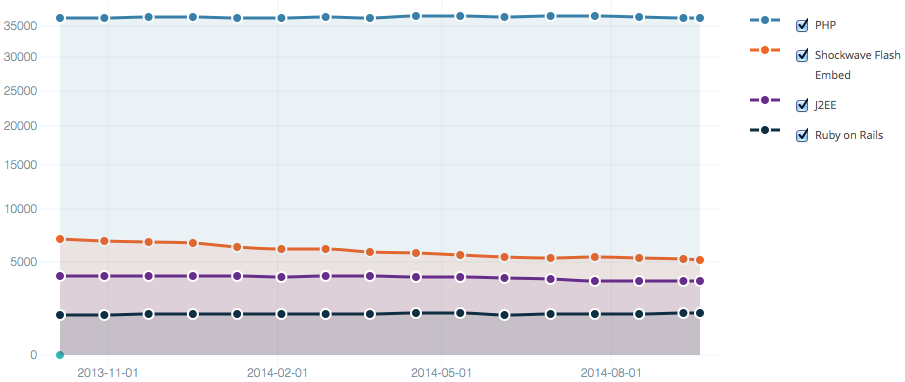
\includegraphics[width=0.618\textwidth]{media/img/EntwicklungVonWebserverTechnologien.png}
				\end{center}
					\caption{Entwicklung von Webserver"=Technologien der Top 10'000 Sites \cite{sharesOfWebtechnologies}}
					\label{fig:EntwicklungVonWebserverTechnologien}
			\end{wrapfigure}
			Schlussendlich haben wir uns da nach Recherchen auf eine "`1"' geeinigt, weil entgegen den Erwartungen von Laurin Murer sich die Verbreitung von PHP (auch von den grösseren Seiten) kaum verändert hat.
			Als Beispiel für eine Technologie die am aussterben ist haben wir Shockwave Flash herangezogen, welche wie man in Abbildung~\ref{fig:EntwicklungVonWebserverTechnologien} sieht im letzten Jahr deutlich an Boden verloren hat.
			Und im Vergleich dazu ist PHP sehr gut im Markt vertreten und hat auch eine äusserst konstante Verbreitung.
			Deshalb sehen wir da auch die Zukunftsaussichten gegeben.
			
			\begin{figure}[H]
				\begin{minipage}[b]{\linewidth}
					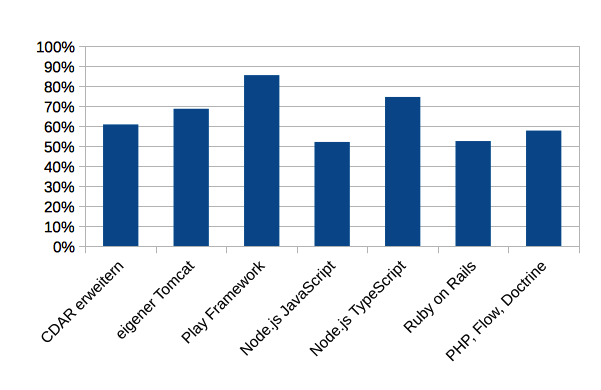
\includegraphics[width=\textwidth]{media/spreadsheets/ServertechnologieVergleichVergleichDerTechnologienDiagramm.png}
					\centering
					\caption{Ergebnis Servertechnologie-Vergleich}
					\label{fig:ErgebnisServertechnologieVergleich}
				\end{minipage}
			\end{figure}
			
			Schlussendlich haben wir für jede Technologie das Total der Punkte berechnet (für jedes Kriterium die Punkte multipliziert mit der Priorität des Kriteriums) und in Abbildung~\ref{fig:ErgebnisServertechnologieVergleich} sieht man das finale Ergebnis. Aufgrund diesem haben wir uns für das Play Framework entschieden. Eine Alternative wäre noch Node.js mit TypeScript gewesen, doch dies hat bereits 10\%-Punkte weniger erreicht.

		\subsubsection{Play Framework}
			Im Kapitel~\ref{serverEvaluation} haben wir erläutert, warum wir das Play Framework ausgewählt haben. Unten die Zusammenfassung, wie Wikipedia das Play Framework beschreibt:
			\begin{quote}
				"`Play is an open source web application framework, written in Scala and Java, which follows the model–view–controller (MVC) architectural pattern. It aims to optimize developer productivity by using convention over configuration, hot code reloading and display of errors in the browser."'\cite{playFrameworkWikipedia}
			\end{quote}
			Um nochmals zusammenzufassen, wir haben es primär aus folgenden Gründen verwendet:
			\begin{itemize}
				\item Das Play Framework basiert auch auf Java, genau so wie das bestehende CDAR.
				\item Ein Teammitglied hat bereits Erfahrungen mit dem Framework gemacht.
				\item Das andere Teammitglied kennt immerhin die zugrundeliegende Sprache (Java).
				\item Der betreuende Dozent hat eine Präferenz für Java.
				\item Das Play Framework benötigt wenig Boilerplate-Code.
				\item Es sprechen keine zwingenden Gründe dagegen (wie beispielsweise zu einschränkende Lizenzen).
				\item Und zu guter Letzt, wir erwarteten Spass am Entwickeln mit dem Play Framework zu haben.
			\end{itemize}

